\chapter{Methodology}\label{chapter:methodology}%Todo change into chapter
In this chapter, the simulator used to investigate the research questions is described. An overview of the system is presented in section \ref{section:systemt architecture}. Section \ref{section:genetic algorithm} includes implementation details, and design decisions made when implementing the genetic algorithm which is the foundation for all the population distributed genetic algorithms. Sections \ref{section:island model}-\ref{section:pool model} contains implementation details of the population distributed genetic algorithms. The wind scenarios used to evaluate the different population distributed genetic algorithm are described in section \ref{section:scenarios}, and the choice of implementing the genetic algorithm from scratch is defended in section \ref{section:motivation}.


\section{System Architecture}\label{section:systemt architecture}
The program is implemented in Java and the interactions between the different classes of the program are shown in figure \ref{figure:class diagram}. The GeneticAlgorithm class is extended by the three population distributed genetic algorithm classes: IslandModel, CellularModel and PoolModel. In addition, the GeneticAlgorithm class is also implemented as instances in all three population distributed algorithms. The main loop of the program is contained in the GeneticAlgorithm class. It uses instances of the classes WindScenario, WindFarmLayoutEvaluator, Population, AdultSelection, ParentSelection, Crossover and Mutation. AdultSelection, ParentSeleciton and Crossover are interfaces that needs to be implemented if new methods are to be added to the program. Mutation is a class containing four different mutation methods. 


\begin{figure}[h!]
\begin{center}
\includegraphics[scale=0.3]{images/"Class Diagram"}
\caption{Class Diagram.}
\label{figure:class diagram}
\end{center}
\end{figure}


\section{Genetic Algorithm}\label{section:genetic algorithm}
As mentioned in \textcolor{red}{reference chapter background}, the genetic algorithm consists of five steps: Adult selection, parent selection, recombination and fitness evaluation as shown in figure \ref{figure:genetic algorithm steps}. The implementation details of each step is described below.


\begin{figure}[h!]
\begin{center}
\includegraphics[scale=0.3]{images/"genetic algorithm steps"}
\caption{Genetic algorithm.}
\label{figure:genetic algorithm steps}
\end{center}
\end{figure}


\subsection{Representation}
As most of the studies from chapter \ref{chapter:relatedwork}, the individuals implemented in the genetic algorithm for this thesis uses a binary representation. However, each position in the binary array can be directly mapped into an integer position which is kept in an array called ''grid''. The purpose behind this design decision is that not all positions in the terrain, when dividing the terrain into a squared grid, are possible turbine positions because the existence of obstacles. By implementing individuals this way, the genetic operations can be performed on individuals without having to check for illegal positions since this is already taken care as soon as the scenario is read from file. Also, this design decision makes sure that no space is wasted in the representation. Figure \ref{figure:representation} shows how the binary representation and ''grid''-array are mapped into a wind farm. \textcolor{red}{Explain the figure when it is made.}. Wind parameters and obstacles positions are read into the program from the scenarios provided by GECCO 2016, these will be described later in this chapter.


\begin{figure}[h!]
\begin{center}
\includegraphics[scale=0.5]{images/"representation program"}
\caption{Individual representation. The grey squares represent legal turbine positions in the terrain, while as the red represent illegal positions. Since there are only nine legal positions in this example, an individual is represented as a binary string of length 9. The grid array is shared between all the individuals and holds the (x, y)-coordinates for each legal position.}
\label{figure:representation}
\end{center}
\end{figure}


\subsection{Adult Selection}\label{subsection:adult selection}
Adult selection is the process of selecting which individuals that are allowed to step into the adult pool and thereby become potential parents for the next generation of individuals. Three adult selection mechanisms were implemented in this thesis: Full generational replacement,  generational mixing, and overproduction. Each method was tested in order to decide which adult selection method was more suitable for solving the wind farm layout optimization problem. \\

\noindent Full generational replacement, is the simplest adult selection mechanism consisting of replacing all the individuals in the previous adult population with the newly generated child population. \\

\noindent The second method, generational mixing, is illustrated in figure \ref{figure:generational mixing}. As can be seen in the figure, the four best individuals (individuals with lowest fitness) from the pool consisting of all the newly generated children and the previous adult population are selected as the new adult population. \\


\begin{figure}[h!]
\begin{center}
\includegraphics[scale=0.2]{images/"adult selection"/"generational mixing"}
\caption{Generational mixing. The best individuals, those with lowest fitness, from the previous adult pool and the new child population are selected to represent the new adult pool.}
\label{figure:generational mixing}
\end{center}
\end{figure}


\noindent Overproduction, the third adult selection mechanism, is illustrated in figure \ref{figure:overproduction}. The newly generated child population consist of twice as many individuals than in the adult pool. Therefore, the child population have to compete against each other for the spots in the adult pool and only those with better fitness are able to survive. \\


\begin{figure}[h!]
\begin{center}
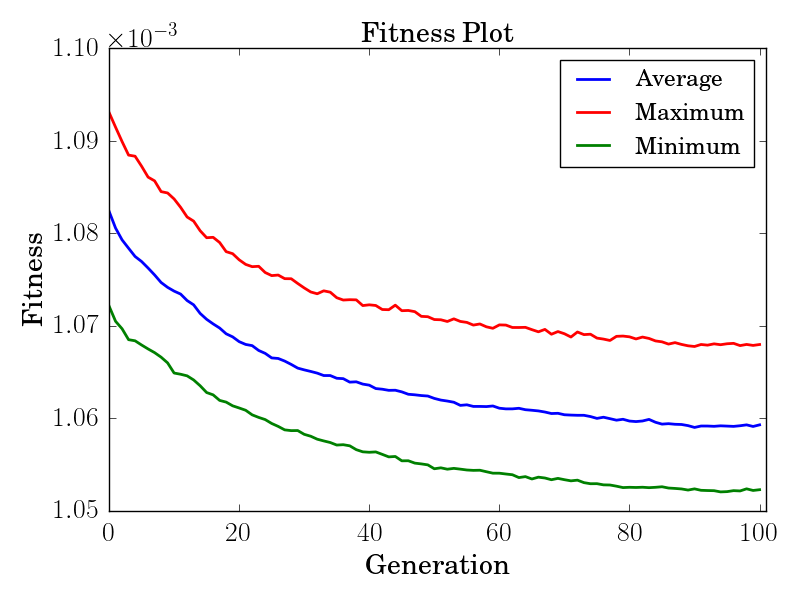
\includegraphics[scale=0.2]{images/"adult selection"/overproduction}
\caption{Overproduction. The newly generated child population consist of twice as many individuals as there are room for in the adult population, therefore only the fittest individuals from the large child population grow up into adults.}
\label{figure:overproduction}
\end{center}
\end{figure}



\subsection{Parent Selection}\label{subsection:parent selection}
Parent selection is the selection of which adults become parents for the next child generation. When choosing parent selection method there are a few concerns that needs to be addressed. First, it is important that parents with good genes, i.e. higher fitness, gets their genes transferred to the next generation. However, it is also important to keep diversity in the population so that one does not end wit a sub-optimal solution; a local maxima. Two parent selection methods are implemented for the genetic algorithm: Tournament selection and roulette wheel selection. \\

\noindent In tournament selection, a given number of individuals are drawn randomly from the population. The number of individuals drawn is decided by the variable ''tournament size''. These individuals compete in a tournament for one spot in the parent pool. The individual with ''best'', i.e. lowest fitness is selected as a parent. These tournaments continue until the adult pool is full. Figure \ref{figure:tournament selection} shows how tournament selection works. As can be seen in the figure, three individuals are drawn randomly from the adult pool, meaning that the tournament size in this example is 3. The ''best'' individual, the individual with fitness 4 is the tournament winner and is allowed to enter the adult pool. \\


\begin{figure}[h!]
\begin{center}
\includegraphics[scale=0.2]{images/"parent selection"/"tournament selection"}
\caption{Tournament selection.}
\label{figure:tournament selection}
\end{center}
\end{figure}


\noindent Different values of ''tournament size'' needs to be tested in order to find how settings that allow the algorithm to explore different solutions, but that also prioritize the best solutions. In chapter \textcolor{red}{reference results chapter}, results obtained for different tournament sizes are compared to find which is best for the wind farm layout optimization problem. \\


\noindent Roulette wheel selection assigns a probability of being chosen as parent to each individuals which is proportional to its fitness compared to all other solutions. Therefore, individuals with better fitness will be more likely to selected for the parent pool. Figure \ref{figure:roulette wheel selection} shows how roulette wheel selection works. The roulette wheel on the left shows the probability of each of the four individuals been selected. Since individual$_4$ has the best fitness, it has a larger probability of being selected than the others. \\


\begin{figure}[h!]
\begin{center}
\includegraphics[scale=0.5]{images/"parent selection"/"roulette wheel selection"}
\caption{Roulette wheel selection. The roulette wheel is shown to the left, the four individuals to the right. Individual$_4$ has a four times better fitness than individual$_2$ and therefore has a four times larger probability of being selected.}
\label{figure:roulette wheel selection}
\end{center}
\end{figure}


\subsection{Genetic Operations}\label{subsection:genetic operations}
This subsection gives an overview over the genetic operations used to produce the next child generation. Three crossover methods, elitism and four mutation methods are implemented and will be presented. 


\subsubsection{Crossover and Elitism}
Crossover is the recombination method utilized by the genetic algorithm to perform sexual reproduction. A crossover operation produced two children by recombining genes of two parent individuals. The genetic algorithm implemented for this thesis has three crossover methods to chose from: Single point crossover, two point crossover and uniform crossover. These are all presented in figure \ref{figure:crossover methods}. As shown in figure \ref{figure:single point crossover}, single point crossover is a method where a random position, called the crossover point, is generated. All genes from the first parent prior to the crossover point are copied to the first child, and all genes after the crossover point are copied to the second child, and all genes from the second parent prior to the crossover point is copied to the second child, and all genes after the crossover point is copied to the first child. Two point crossover is similar to single point crossover, except that it uses to crossover points instead of one. This is shown in figure \ref{figure:two point crossover}. In uniform crossover, there is a fifty percent probability that each gene will be drawn from each parent as shown in figure \ref{figure:uniform crossover}. This crossover method results in child individuals that might not inherit the gene patterns from their parents the same way as in the other two methods. Since the relative positions between wind turbines are very important when solving the wind farm layout optimization problem, uniform crossover might not be the best choice. \textcolor{red}{Is this true? If it is, talk about this in the results part, remove it from here.}


\begin{figure}[h!]
    \centering
    \begin{subfigure}[b]{0.3\textwidth}
        \includegraphics[width=\textwidth]{images/crossover/"Single point crossover"}
        \caption{Single point crossover.}
        \label{figure:single point crossover}
    \end{subfigure}
    ~ 
    \begin{subfigure}[b]{0.3\textwidth}
        \includegraphics[width=\textwidth]{images/crossover/"Two point crossover"}
        \caption{Two point crossover.}
        \label{figure:two point crossover}
    \end{subfigure}
    ~
    \begin{subfigure}[b]{0.3\textwidth}
        \includegraphics[width=\textwidth]{images/crossover/"Uniform crossover"}
        \caption{Uniform crossover.}
        \label{figure:uniform crossover}
    \end{subfigure}
    \caption{Crossover methods.}\label{figure:crossover methods}
\end{figure}


\subsubsection{Mutation}
Although crossover is a powerful genetic operator, which able child individuals to inherit genes from the best parent individuals, it is not enough on its own. Without any way to mutate genes, one can end up with a population where every individual has the same gene value in the same position, this means that no recombination will be able to change the value of that gene. Mutation is the operation used by the genetic algorithm to make sure that the population do not get sterile. In nature, genes can be mutated in numerous ways. In this thesis, four mutation methods are implemented to mimic the mutations methods that can happen in genes, these are called: Flip mutation, 


\subsection{Wind-, Wake- and Power Model}\label{subsection:wind-, wake- and power model}
The evaluation class uses the same wake-, wind- and power model as \cite{Kusiak}. The wake model used is the classical Jensen model \citep{Jensen}, which is used in almost every study of the wind farm layout optimization problem, as can be seen in table \ref{table:overview}. \\

\noindent Wind distribution is modeled using the Weibull distribution, a continuous probability distribution shown to model wind distribution quite well \citep{Justus}. The probability density function is shown in equation \ref{equation:Weibull}


\begin{equation}
f(x; c, k)  = 
\begin{cases}
\frac{k}{c} \left( \frac{x}{c} \right)^{k-1} e^{- \left( \frac{x}{c} \right)^k } & \text{if} \hspace{1mm} x \geq 0 \\
0                                                                                                                      & \text{if} \hspace{1mm}     x < 0
\end{cases}
\label{equation:Weibull}
\end{equation}


\noindent where $k$ is called the shape parameter and $c$ is the scale parameter, and $k, c > 0$. In most of the wind scenarios provided by GECCO 2015, $k \approx 2$, this is shown empirically to be a good value for wind speed distribution \citep{Justus}. On the other hand, the shape parameter vary for each wind direction. Figure \ref{figure:weibull distribution} shows the Weibull distribution plotted for $k = 2$ and for different values of $c$. \\


\begin{figure}[h!]
\begin{center}
\includegraphics[scale=0.4]{images/"Weibull"}
\caption{The Weibull distribution plotted for $k = 2$ for different values of the scale parameter $c$.}
\label{figure:weibull distribution}
\end{center}
\end{figure}

\noindent The wind scenarios used in this thesis are therefore a specification of the shape- and scale parameters for every wind direction, where wind direction is partitioned into 24 different directions. Twenty wind scenarios are provided by GECCO 2015, ten which simply specify wind distribution parameters, and ten that specify wind distribution parameters and locations of obstacles. \\

\noindent The power curve used is also the same as used in \cite{Kusiak}, it is a linear function, shown in equation \ref{equation:Power Curv (API)},

\begin{equation}
 f(v) = 
  \begin{cases} 
   0                                  & \text{if }     v < v_{cut-in} \\
   \lambda v + \eta           & \text{if }     v_{cut-in} \leq v \leq v_{rated} \\
   P_{rated}                        & \text{if }     v_{cut-out} > v > v_{rated}. \\
  \end{cases}
  \label{equation:Power Curv (API)}
\end{equation}

\noindent Here $\lambda$ is the slope parameter, $v$ the wind speed, $\eta$ the intercept parameter, $P_{rated}$ is the fixed power output, and $v_{cut-in}$ is the cut-in speed; the minimum speed for which the turbine produces power, and $v_{cut-out}$ is the cut-out speed; the maximum wind speed for which the turbine is kept on. 


\subsection{Fitness Function}\label{subsection:fitness function}
The main task of the evaluation classes is to calculate the fitness of each individual based on the fitness function.  The fitness function to be optimized is provided by GECCO, and is displayed in equation \ref{Objective function}.\\

\begin{small}
\begin{equation}
fitness =  \frac{ \left( c_t \cdot n + c_s \cdot \floor*{\frac{n}{m}} \right) \left( \frac{2}{3} + \frac{1}{3} \cdot e^{-0.00174n^2} \right) + c_{OM} \cdot n}{\left( \frac{1 - (1 + r)^{-y}}{r} \right) } \cdot \frac{1}{8760 \cdot P} + \frac{0.1}{n}
\label{Objective function} 
\end{equation}
\end{small}


\noindent Description and numerical values of all parameters given in equation \ref{Objective function} are displayed in table \ref{Parameters}. As can be seen in this table, the values of $n$, the number of turbines, and $P$, farm energy output, are not given. This is because the number of turbines, together with the turbine positions, are the parameters to be optimized by the genetic algorithm. Farm energy output is the indirect parameter that we are trying to optimize. It is dependent on turbines count, position, wind scenario and so on, and is off course therefore not provided in table \ref{Parameters} either.\\


\begin{table}[h!]
\begin{center}
\caption{Description and value of each parameter used in the objective function provided by GECCO 2015.}
\label{Parameters}
\begin{tabular}{l|l|l}
\textbf{Parameter} & \textbf{Description} & \textbf{Value} \\ 
\hline 
$c_t$ & Turbine cost (usd) & 750 000 \\ 
$c_s$ & Substation cost (usd) & 8 000 000 \\ 
$m$ & Turbines per substation & 30 \\ 
$r$ & Interest rate & 0.03 \\ 
$y$ & Farm lifetime (years) & 20 \\ 
$c_{OM}$ & Yearly operating costs per turbine & 20 000 \\ 
$n$ & Number of turbines &  \\ 
$m$ & Farm energy output &  \\  
\end{tabular} 
\end{center}
\end{table}


\noindent Intuitively, the objective function can be divided into different parts. The first parenthesis in the nominator of the first fraction is the construction cost, while the second parenthesis is the economies of scale and the third part of the nominator is yearly operating costs. The denominator represents the interests. The denominator of the second fraction describes yearly power output, while the number $0.1$ in the nominator of the last fraction is a farm size coefficient. \\


\section{Island Model}\label{section:island model}


\section{Cellular Model}\label{section:cellular model}


\section{Pool Model}\label{section:pool model}


\section{Scenarios}\label{section:scenarios}


\section{Motivation}\label{section:motivation}